\paragraph{Desarrollo técnico}
Como intento de mejora a la anterior versión, la cual era de conversión directa, se trató de diseñar un receptor superheterodino. A su vez, se mantuvo el diseño del transmisor a varactores, pero se cambió la frecuencia de trabajo a una mayor, unos \SI{6}{\mega\hertz}. 
\paragraph{}
El diseño consistía en un filtro de entrada que era mezclado en un mezclador con un oscilador. Después se realizaba el tratamiento con la señal de frecuencia intermedia. Un amplificador de dos etapas y posteriormente a un rectificador con filtro paso bajo para demodular la señal. Se muestra un esquemático en la figura \ref{fig:crono_sch_receiver_varactor} del receptor sin la parte digital, la cual se explica en el apartado \ref{sec:crono_digital}. La figura \ref{fig:crono_sch_receiver_varactor}, consta de la parte de RF explicada a la derecha, y de la interfaz con la parte digital, un amplificador con realimentaci\'on positiva denominado \textit{Smith-trigger}.

\begin{figure}[h!]
    \centering
    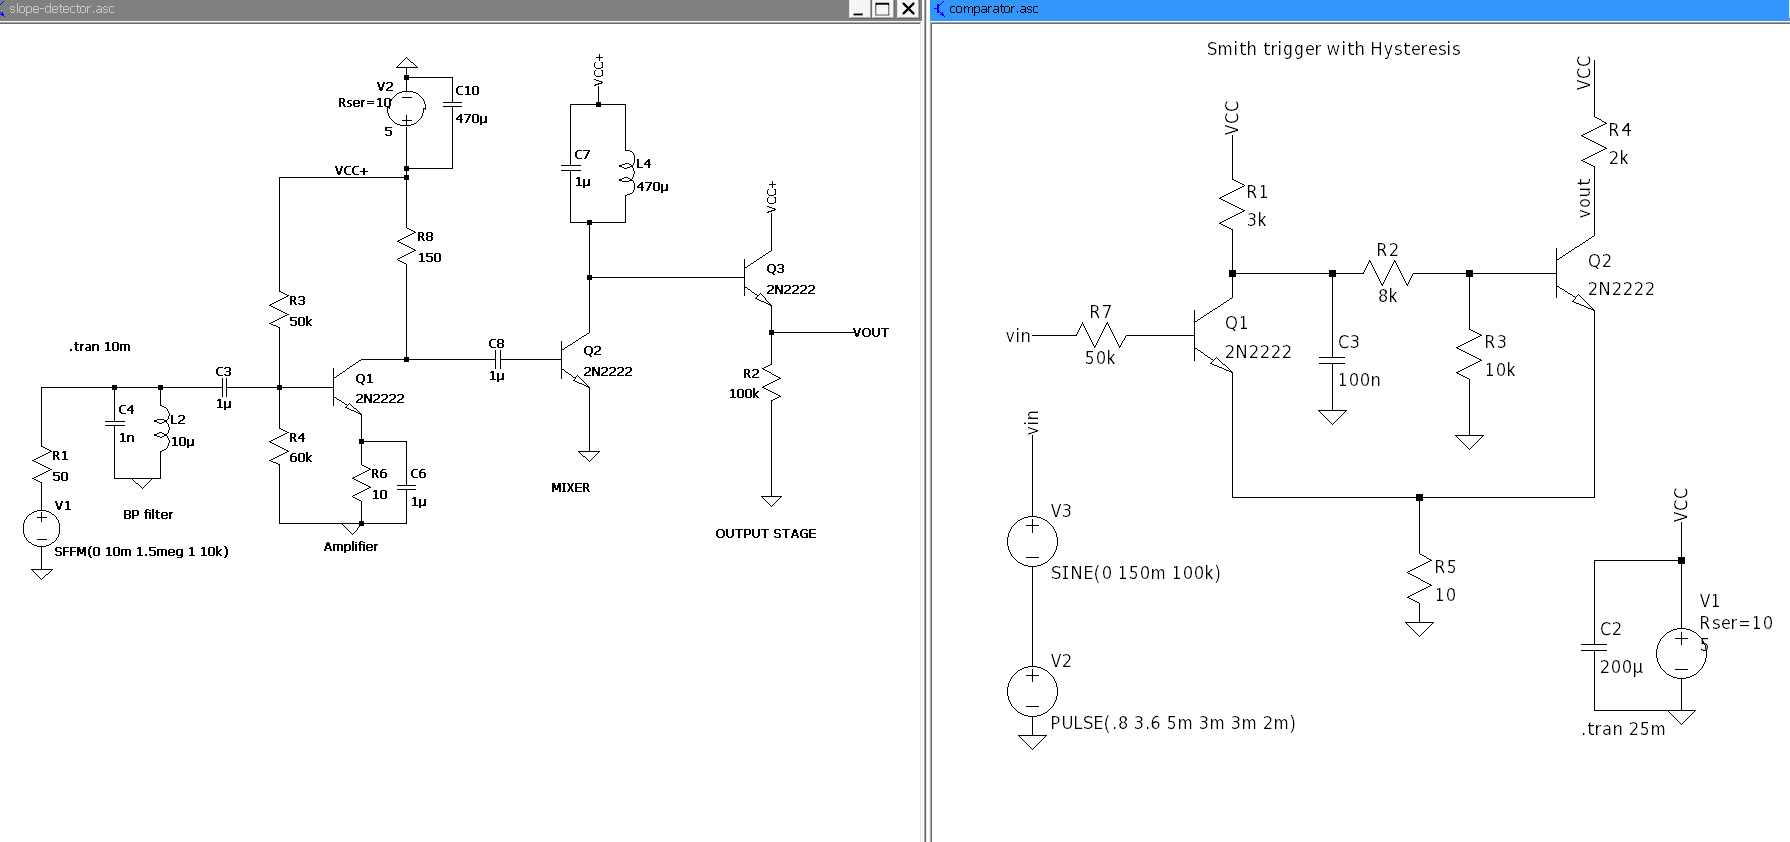
\includegraphics[scale=1, width=1\textwidth]{crono_sch_receiver_varactor}
    \caption{Modelo esquem\'atico del receptor superheterodino de FM}
    \label{fig:crono_sch_receiver_varactor}
\end{figure}

\paragraph{Motivos de reemplazo}
Este diseño funcionaba bien cuando se conectaba a la entrada un generador de frecuencias a la frecuencia de trabajo de muy baja potencia.
\paragraph{}
El problema surgía cuando se trataba de probar con el transmisor. 
El receptor no tenía buena selectividad y los amplificadores de frecuencia intermedia, los cuales no estaban correctamente diseñados, producían oscilaciones.
\paragraph{}
Gracias al mezclador, el circuito era capaz de detectar señales de muy baja potencia con muy buena selectividad. A pesar de todo, el mezclador era bastante sensible al ruido, ya que producía bastantes armónicos, producidos por efectos de segundo orden. Esto explica el por qué al conectarlo con el generador, lo más cercano a un tono puro, funcionaba correctamente, sin embargo cuando se trataba de enlazar con la señal del transmisor la cosa cambiaba.
\paragraph{}
También, el diseño general, me parecía que se utilizaban demasiados componentes para unas prestaciones tan bajas. El diseño debía ser sencillo y funcional.
\paragraph{}
Debido a la complejidad a cambio de ninguna clase de beneficio, se opta por transicionar a un esquema de modulaci\'on AM.
